\documentclass{article} 
\documentclass[UTF8]{ctexart}
\usepackage{xcolor}
\usepackage[colorlinks,linkcolor=blue,anchorcolor=blue,citecolor=blue]{hyperref}
\usepackage{subfigure}
\usepackage{geometry}

\setlength{\parindent}{0pt}

\title{Parallel Programming Test 1}
\author{Name:liukanglai  \qquad Student ID:2019011777}
\date{May 2021}

%\text {Please hand in the PDF version of the test paper.}

\usepackage{natbib}
\usepackage{graphicx}

\begin{document}

\maketitle
$$(Please\ hand\ in\ a\ PDF\ version.)$$

\section{What is parallel computing? (no more than 50 words)}
(Source: 新竹清华大学:并行计算与并行编程课程(周志远教授,2018年秋季学期)\url{https://www.bilibili.com/video/BV1Yt411W7td} Lecture 1C (0:04:50))

Ans:%input your answer here
~\\ Parallel computing is a type of computation in which many calculations or processes are carried out at the same time.

\section{What is a supercomputer? How can the performance of supercomputers be measure? (no more than 100 words)}
(Source: 新竹清华大学:并行计算与并行编程课程(周志远教授,2018年秋季学期)\url{https://www.bilibili.com/video/BV1Yt411W7td} Lecture 3A (0:06:14))

Ans:%input your answer here
~\\ A supercomputer is a computer with a high level of performance than a general-purpose computer. It has more cores and more other better hardware.
Use GFlops(floating point ) to measure it.

\section{Talk about your understanding of the Strong scaling and the Weak scaling. (no more than 50 words)}
(Source: UC Berkeley CS267 Applications of Parallel Computers (Kathy Yelick et al., Spring 2018) \url{https://www.bilibili.com/video/BV1qV411q7RS} Lecture 1 Introduction (1:13:31))

Ans:%input your answer here
~\Amdahl’s Law — Strong Scaling •Fixed Problem Size •How much does parallelism reduce the execution time of a problem?  • 
Gustafson’s Law — Weak Scaling
•Fixed Execution Time
•How much longer does it take for the problem without parallelism?\

\section{What do compilers do for languages like C/C++ and Fortran? (no more than 50 words)}
(Source: UC Berkeley CS267 Applications of Parallel Computers (Kathy Yelick et al., Spring 2018) \url{https://www.bilibili.com/video/BV1qV411q7RS} Lecture 2 (0:11:28))

Ans:%input your answer here
~\\ It translates (compiles) source code  into a set of machine-language instructions that can be understood by a digital computer's CPU.
\section{Can we expand the size of the cache indefinitely? Why is that? (no more than 100 words)}
\textcolor{blue}{Tips: Cache is a really fast type of memory. A computer has multiple levels of memory. The first is primary storage, which could be a hard disk or an SSD storing the heavy data like your operating system and programs. Next is the RAM, can be much faster than your primary storage. Lastly you have cache, which comprises of the even faster memory units closer to compute units (e.g., ALUs).}

(Source: UC Berkeley CS267 Applications of Parallel Computers (Kathy Yelick et al., Spring 2018) \url{https://www.bilibili.com/video/BV1qV411q7RS} Lecture 2 (0:31:38))

Ans:%input your answer here
~\\
no
\section{Talk about your understanding of spatial locality and temporal locality of cache. (no more than 50 words)}
(Source: UC Berkeley CS267 Applications of Parallel Computers (Kathy Yelick et al., Spring 2018) \url{https://www.bilibili.com/video/BV1qV411q7RS} Lecture 2 (0:22:30))

Ans:%input your answer here
~\ Temporal locality refers to the reuse of specific data and/or resources within a relatively small time duration. Spatial locality (also termed data locality) refers to the use of data elements within relatively close storage locations.\
\section{The following two figures are Roofline models of a generic machine. The left figure considers the computation of multiple optimization methods, and the right one adds bandwidth considerations. Please analyze the content of the two figures. (no more than 200 words)}

\begin{figure}[htbp]
\centering
\subfigure[]{
    \begin{minipage}[t]{0.4\linewidth}
    \centering
    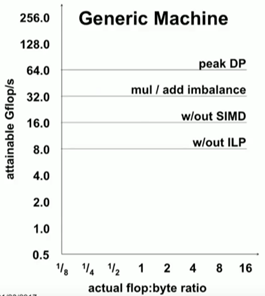
\includegraphics[width=2in]{roofline(a).png}
    \end{minipage}
}
\subfigure[]{
    \begin{minipage}[t]{0.4\linewidth}
    \centering
    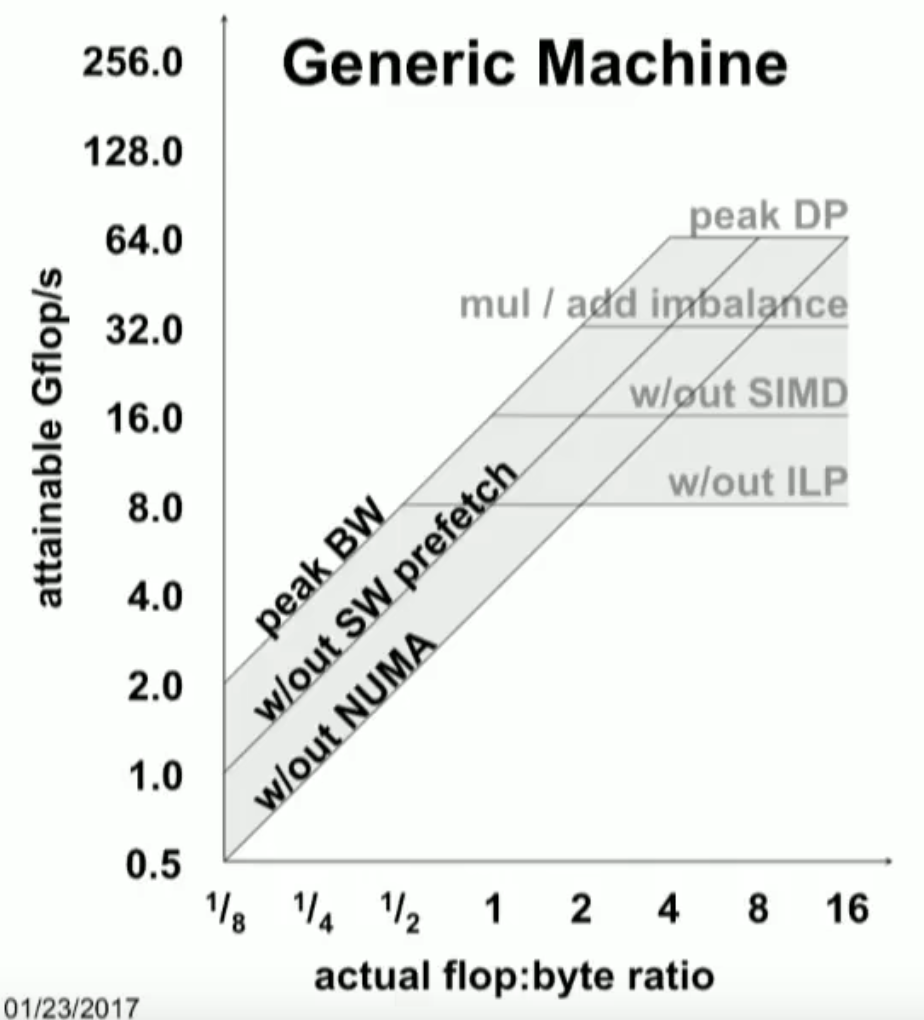
\includegraphics[width=2in]{roofline(b).png}
    \end{minipage}
}
\end{figure}

(Source: UC Berkeley CS267 Applications of Parallel Computers (Kathy Yelick et al., Spring 2018) \url{https://www.bilibili.com/video/BV1qV411q7RS} Lecture 2 (0:48:23))

Ans:%input your answer here
~\\
no
\section{Please draw a figure to explain the blocked (tiled) algorithm for General Matrix-Matrix Multiplication (GEMM). (Take a photo and attach the photo)}
(Source: UC Berkeley CS267 Applications of Parallel Computers (Kathy Yelick et al., Spring 2018) \url{https://www.bilibili.com/video/BV1qV411q7RS} Lecture 2 (1:15:50))

Ans:%upload your photo and insert it
\begin{figure}[ht]
\centering

\includegraphics[width=5in]{example.png}
%\caption{example}
\end{figure}


\section{Here are two pieces of GEMM code in different loop orders. Which one do you think has the better performance? And why? (no more than 100 words)}
\begin{figure}[htbp]
\centering
\subfigure[]{
    \begin{minipage}[t]{0.4\linewidth}
    \centering
    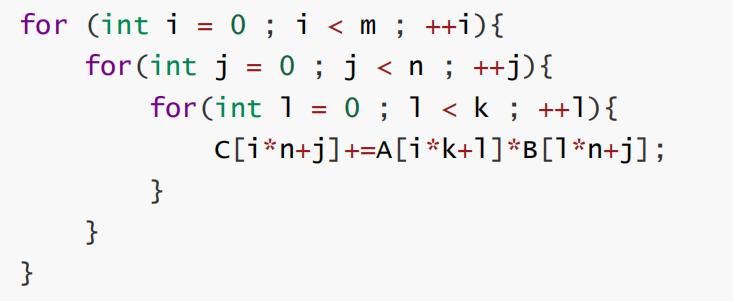
\includegraphics[width=2.5in]{a.png}
    \end{minipage}
}
\subfigure[]{
    \begin{minipage}[t]{0.4\linewidth}
    \centering
    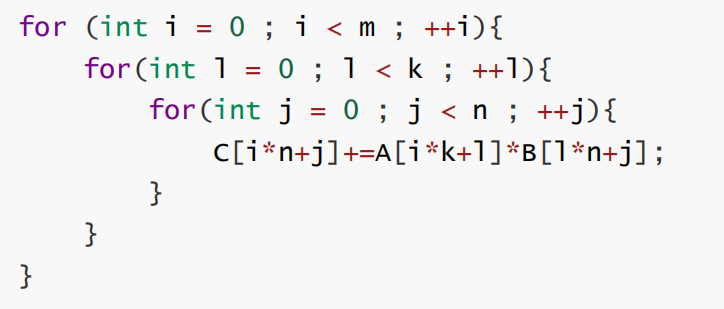
\includegraphics[width=2.5in]{b.png}
    \end{minipage}
}
\end{figure}

(Source: homework 1)

Ans:%input your answer here
~\\
no
The second code is better than the first.Because the number in matrix A and B move closer.
\section{Please describe the function of statements \texttt{\#pragma omp barrier} and \texttt{\#pragma omp task}. (no more than 50 words)}
(Source: UC Berkeley CS267 Applications of Parallel Computers (Kathy Yelick et al., Spring 2018) \url{https://www.bilibili.com/video/BV1qV411q7RS} Lecture 4 (1:13:00) and homework 2)

Ans:%input your answer here
~\\It will wait untill all the thread get the barrier, and then all the thread will carry out the part after the barrier.
Use the task pragma when you want to identify a block of code to be executed in parallel with the code outside the task region. The task pragma can be useful for parallelizing irregular algorithms such as pointer chasing or recursive algorithms. The task directive takes effect only if you specify the SMP compiler option.

\bibliographystyle{plain}
\end{document}
